\documentclass{article}

% Packages for formatting
\usepackage[margin=1in]{geometry}
\usepackage{fancyhdr}
\usepackage{enumitem}
\usepackage{graphicx}
\usepackage{kotex}
\usepackage{amsmath}
\usepackage{amsthm}
\usepackage{algorithm2e,setspace}
\usepackage{algpseudocode}
\usepackage{xcolor}
\usepackage{amssymb}

% Fonts
\usepackage[T1]{fontenc}
\usepackage[utf8]{inputenc}
\usepackage{newpxtext,newpxmath}
\usepackage{sectsty}

% Define colors
\definecolor{blue1}{HTML}{0077c2}
\definecolor{blue2}{HTML}{00a5e6}
\definecolor{blue3}{HTML}{b3e0ff}
\definecolor{blue4}{HTML}{00293c}
\definecolor{blue5}{HTML}{e6f7ff}

\definecolor{thmcolor}{RGB}{231, 76, 60}
\definecolor{defcolor}{RGB}{52, 152, 219}
\definecolor{lemcolor}{RGB}{155, 89, 182}
\definecolor{corcolor}{RGB}{46, 204, 113}
\definecolor{procolor}{RGB}{241, 196, 15}

\usepackage{color,soul}
\usepackage{soul}
\newcommand{\mathcolorbox}[2]{\colorbox{#1}{$\displaystyle #2$}}
\usepackage{cancel}
\newcommand\crossout[3][black]{\renewcommand\CancelColor{\color{#1}}\cancelto{#2}{#3}}
\newcommand\ncrossout[2][black]{\renewcommand\CancelColor{\color{#1}}\cancel{#2}}

\usepackage{hyperref}
\usepackage{booktabs}

% Chapter formatting
\definecolor{titleblue}{RGB}{0,53,128}
\usepackage{titlesec}
\titleformat{\section}
{\normalfont\sffamily\Large\bfseries\color{titleblue!100!gray}}{\thesection}{1em}{}
\titleformat{\subsection}
{\normalfont\sffamily\large\bfseries\color{titleblue!50!gray}}{\thesubsection}{1em}{}

%Tcolorbox
\usepackage[most]{tcolorbox}

%Tikzpicture
\usepackage{tikz-cd}
\usetikzlibrary{positioning}
\usetikzlibrary{angles, quotes}

% Header and footer formatting
\pagestyle{fancy}
\fancyhead{}
\fancyhf{}
\rhead{Student ID: 20192250\quad Name: 지용현}%\rule{3cm}{0.4pt}}
\lhead{\textcolor{blue2}{\textbf{CA Assignment \#2}}}
% Define footer
\newcommand{\footer}[1]{
\begin{flushright}
	\vspace{2em}
	
\includegraphics[width=2cm]{school_logo.jpg} \\
	\vspace{1em}
	\textcolor{blue2}{\small\textbf{#1}}
\end{flushright}
}
%\rfoot{\large Department of Information Security, Cryptogrphy and Mathematics, Kookmin Uni.
\includegraphics[height=1.5cm]{school_logo.jpg}}
\fancyfoot{}
\fancyfoot[C]{-\thepage-}

\newcommand{\ie}{\textnormal{i.e.}}
\newcommand{\rsa}{\mathsf{RSA}}
\newcommand{\rsacrt}{\mathsf{RSA}\textendash\mathsf{CRT}}
\newcommand{\inv}[1]{#1^{-1}}

\usepackage{amsthm}
\newtheorem{axiom}{Axiom}[section]
\newtheorem{theorem}{Theorem}
\newtheorem*{theorem*}{Theorem}
\newtheorem{proposition}[theorem]{Proposition}
\newtheorem{corollary}{Corollary}[theorem]
\newtheorem*{corollary*}{Corollary}
\newtheorem{lemma}[theorem]{Lemma}
\newtheorem*{lemma*}{Lemma}

\theoremstyle{definition}
\newtheorem{definition}{Definition}
\newtheorem*{definition*}{Definition}
\newtheorem{remark}{Remark}
\newtheorem{exercise}{Exercise}[section]

%New Command
\newcommand{\set}[1]{\left\{#1\right\}}
\newcommand{\N}{\mathbb{N}}
\newcommand{\Z}{\mathbb{Z}}
\newcommand{\Q}{\mathbb{Q}}
\newcommand{\R}{\mathbb{R}}
\newcommand{\C}{\mathbb{C}}
\newcommand{\F}{\mathbb{F}}
\newcommand{\nbhd}{\mathcal{N}}
\newcommand{\Log}{\operatorname{Log}}
\newcommand{\Arg}{\operatorname{Arg}}
\newcommand{\pv}{\operatorname{P.V.}}

\newcommand{\of}[1]{\left( #1 \right)} 
\newcommand{\abs}[1]{\left\lvert #1 \right\rvert}
\newcommand{\norm}[1]{\left\| #1 \right\|}

\newcommand{\sol}{\textcolor{magenta}{\bf Sol}}
\newcommand{\conjugate}[1]{\overline{#1}}


\renewcommand{\Re}{\operatorname{Re}}
\renewcommand{\Im}{\operatorname{Im}}

\begin{document}
\pagenumbering{arabic}
\begin{center}
	\huge\textbf{Complex Analysis}\\
	\vspace{0.5em}
\end{center}

\begin{enumerate}
	\item We define \[
	f'\of{t}=\frac{d}{dt}\left[u\of{t}+iv\of{t}\right] = u'\of{t}+iv'\of{t},\quad
	\int f\of{t}dt = \int u\of{t}dt + i\int v\of{t}dt.
	\] \begin{itemize}
		\item[(a)]
		\item[(b)]
		\item[(c)]
	\end{itemize}
	\begin{proof}[\sol]
		\begin{itemize}
			\item[(a)] Note that \[
			f\of{t}=e^{z_0t}=e^{\of{a+ib}t}=e^{at}e^{i bt}=e^{at}\of{\cos\of{bt}+i\sin\of{bt}}.
			\] Then \begin{align*}
				u\of{t} &=\Re\of{e^{z_0t}}=e^{at}\cos\of{bt},\\
				v\of{t} &=\Im\of{e^{z_0t}}=e^{at}\sin\of{bt},
			\end{align*} and so \begin{align*}
				u'\of{t}=\frac{d}{dt}\left[e^{at}\cos\of{bt}\right]&=ae^{at}\cos\of{bt}-be^{at}\sin\of{bt},\\
				v'\of{t}=\frac{d}{dt}\left[e^{at}\sin\of{bt}\right]&=ae^{at}\sin\of{bt}+be^{at}\cos\of{bt}.
			\end{align*} Thus \begin{align*}
				f'\of{t}=u'\of{t}+iv'\of{t}&=ae^{at}\cos\of{bt}-be^{at}\sin\of{bt}+iae^{at}\sin\of{bt}+ibe^{at}\cos\of{bt}\\
				&=ae^{at}\cos\of{bt}-i^2be^{at}\sin\of{bt}+iae^{at}\sin\of{bt}+ibe^{at}\cos\of{bt}\\
				&=(ae^{at}+ibe^{at})\of{\cos\of{bt}+i\sin\of{bt}}\\
				&=\of{a+bi}\cdot e^{at}e^{ibt}\\
				&=\of{a+bi}e^{\of{a+bi}t}\\
				&=z_0e^{z_0t}.
			\end{align*}
			\item[(b)] \[
			\int e^{z_0t}dt = \frac{1}{z_0}e^{z_0t}=\frac{1}{a+bi}e^{\of{a+bi}t}.
			\]\begin{align*}
				\int e^{z_0t}dt&=\int e^{at}\cos\of{bt}dt +i\int e^{at}\sin\of{bt}dt\\
				&=\int e^{at}\cos\of{bt}dt +i\int e^{at}\sin\of{bt}dt\\
			\end{align*}\begin{align*}
				\int e^{at}\cos(bt)dt &= \frac{1}{2}\int e^{at}\left(e^{ibt} + e^{-ibt}\right)dt \\
				&= \frac{1}{2}\left[\frac{1}{a+ib}e^{(a+ib)t} + \frac{1}{a-ib}e^{(a-ib)t}\right] + C \\
				&= \frac{1}{2}\left[\frac{(a-ib)e^{(a+ib)t} + (a+ib)e^{(a-ib)t}}{a^2 + b^2}\right] + C \\
				&= \frac{a}{a^2 + b^2}\cdot\frac{1}{2}\left[e^{(a+ib)t} + e^{(a-ib)t}\right] + \frac{b}{a^2 + b^2}\cdot\frac{1}{2i}\left[e^{(a+ib)t} - e^{(a-ib)t}\right] + C
			\end{align*}
			\item[(c)] Note that \begin{align*}
				\frac{1}{a+bi}e^{\of{a+bi}t}&=\frac{1}{a+bi}e^{at}\of{\cos\of{bt}+i\sin\of{bt}}\\
				&=\frac{1}{a+bi}e^{at}\cos\of{bt}+\frac{1}{b-ai}e^{at}\sin\of{bt}\\
				&=
			\end{align*}
			\begin{align*}
				\int e^{z_0t}dt=\int e^{at}\cos\of{bt}+i\int e^{at}\sin\of{bt}\\
			\end{align*}
		\end{itemize}
	\end{proof}
	\item Let $C$ be the path in the complex plane defined as the counter-clockwise rotation of a circle with center at the origin and radius $2$, represented by the function $z(t) = 2e^{it}$ for $t \in [0, 2\pi]$. Calculate the value of the following integral:
	\begin{figure}[h!]
		\centering
		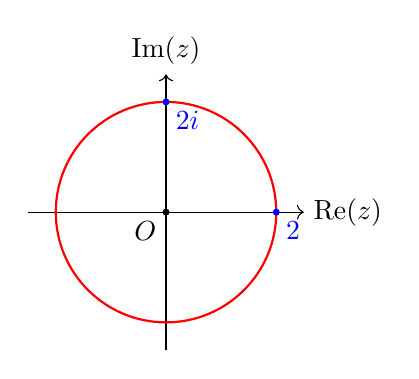
\begin{tikzpicture}[scale=0.7]
			\draw[->] (-2.5,0) -- (2.5,0) node[right] {$\Re(z)$};
			\draw[->] (0,-2.5) -- (0,2.5) node[above] {$\Im(z)$};
			\draw[thick,red] (2,0) arc (0:360:2);
			\filldraw[black] (0,0) circle (1.5pt) node[anchor=north east] {$O$};
			\filldraw[blue] (2,0) circle (1.5pt) node[anchor=north west] {$2$};
			\filldraw[blue] (0,2) circle (1.5pt) node[anchor=north west] {$2i$};
		\end{tikzpicture}
	\end{figure}
	\begin{itemize}
		\item[(a)] $\displaystyle\int_C\frac{e^z}{z}dz$\quad(b) $\displaystyle\int_C\frac{z^2}{z-1}dz$\quad(c) $\displaystyle\int_C\frac{z}{z-3}dz$\quad(d) $\displaystyle\int_C\frac{\cos z}{z\of{z^2+9}}dz$
	\end{itemize}
	\begin{proof}[\sol]
		\begin{itemize}
			\item[(a)] Let $f\of{z}=e^z$ then \[
			\int_C\frac{e^z}{z}dz=\int_C\frac{f\of{z}}{z-0}dz=f\of{0}2\pi i=2\pi i.
			\]
			\item[(b)] Let $f\of{z}=z^2$ then \[
			\int_C\frac{z^2}{z-1}dz=\int_C\frac{f\of{z}}{z-1}dz=f\of{1}2\pi i=2\pi i.
			\]
			\item[(c)] $\displaystyle\int_C\frac{z}{z-3}dz$
			\item[(d)] $\displaystyle\int_C\frac{\cos z}{z\of{z^2+9}}dz$
		\end{itemize}
	\end{proof}
	\item 
	\begin{proof}[\sol]
		content...
	\end{proof}
	\item Find the following integral. \begin{itemize}
		\item[(a)] $\displaystyle\int_0^{2\pi}e^{e^{i\theta}}d\theta$.
		\item[(b)] $\displaystyle\int_0^{2\pi}e^{-i\theta}e^{e^{i\theta}}d\theta$.
	\end{itemize}
	\begin{proof}[\sol]
		Recall that Cauchy integral formula for a function $f\of{z}$ that is analytic inside and on a simple closed contour $C$: \[
		f\of{z_0}=\frac{1}{2\pi i}\oint_C\frac{f\of{z}}{z-z_0}dz.
		\]
		\vspace{4pt}
		\begin{itemize}
			\item[(a)] Let $z = e^{i\theta}$ and $dz = ie^{i\theta} d\theta$ (\ie, $d\theta=\frac{1}{ie^{i\theta}}dz$). Then, the integral becomes: \[
			\int_0^{2\pi}e^{e^{i\theta}}d\theta=\oint_{\abs{z}=1}\frac{e^z}{iz}dz.
			\] Here, the contour $C$ is the unit circle $|z|=1$. The integrand has a simple pole at $z=0$. Using the Cauchy integral formula, we can identify the function $f(z) = e^z$ and $z_0=0$. Thus, the integral is equal to:
			\[
			\int_0^{2\pi}e^{e^{i\theta}}d\theta = \oint_{\abs{z}=1}\frac{e^z}{iz}dz = 2\pi i\cdot f\of{z}=2\pi i\cdot e^0 = 2\pi i.
			\]
			\vspace{4pt}
			\item[(b)] Let $z = e^{i\theta}$ and $dz = ie^{i\theta} d\theta$ (\ie, $d\theta=\frac{1}{ie^{i\theta}}dz$). Then, the integral becomes: \[
			\int_0^{2\pi}e^{-i\theta}e^{e^{i\theta}}d\theta=\oint_{\abs{z}=1}\frac{e^z}{iz^2}dz.
			\] 
		\end{itemize}
	\end{proof}
	\item 
	\begin{proof}[\sol]
		content...
	\end{proof}
	\item 
	\begin{proof}[\sol]
		content...
	\end{proof}
\end{enumerate}

\footer{Department of Information Security, Cryptography and Mathematics, Kookmin University}
\end{document}
